\renewcommand{\vec}{\overline}
\chapter{Геометрия}

\section{Пересечение прямых}
Прямую можно задать уравнением прямой: $a_1x + b_1y + c_1 = 0$ 

Тогда, что бы пересечь прямую нужно решить систему уравнений. 

\begin{gather*}
a_1 x + b_1 y + c_1 = 0\\
a_2 x + b_2 y + c_2 = 0
\end{gather*}

Решим систему:
\begin{enumerate}
\item Если $a_1 b_2 - a_2 b_1 = 0$, то прямые параллельны.
    \begin{enumerate}
    \item Если $a_1 c_2  - c_1 a_2 = 0 \Ra$ прямые совпадают.
    \item в ином случае не совпадают и пересечений нет. 
    \end{enumerate}
\item 
    Определим функцию 
    
    $$\det A = \det (\begin{pmatrix} a_{11} & a_{12}\\ a_{21} & a_{22} \end{pmatrix}) = 
    = a_{11}a_{22} - a_{12}a_{21}$$ 
   
    $$det2(a_{11}, a_{12}, a_{21}, a_{22})$$
   
    $$y = - \frac{det2(A_1, A_2, C_1, C_2)}{det2(A_1, A_2, B_1, B_2)}$$
\end{enumerate}

Многие говорят, что это клево и удобно, но Женя так делать не любит.

Зададим прямую с помощью точки($P$) и вектора($S$).

Тогда любая точка на прямой задается как $P + S \cdot t$

Тогда прямые пересекаются, если
$$p_1 + s_1 t_1 = p_2 + s_2 t_2$$

\begin{Def}
Скалярное произведение: $\vec{a} \cdot \vec{b} = |\vec{a}||\vec{b}|\cos(\angle \vec{a}, \vec{b}) = a_x b_x + a_y b_y$
\end{Def}

\begin{Def}
Псевдовекторное произведение: $\vec{a} \times \vec{b} = |\vec{a}||\vec{b}| \sin(\angle \vec{a}, \vec{b}) = a_x b_y - a_y b_x = det2(a_x, a_y, b_x, b_y)$
\end{Def}

Умеем проверять, являются ли вектора перпендикулярными или коллинеарными. 

Важно помнить, что $\vec{a} \times \vec{b} \ne \vec{b} \times \vec{a}$, более того $\vec{a} \times \vec{b} = -\vec{b} \times \vec{a}$

Можно доказать, что $\vec{a} \times (\vec{b} + \vec{c}) = \vec{a} \times \vec{b} + \vec{a} \times \vec{b}$

$$p_1 \times s_2 + (s_1 \times s_2) t_1 = p_2 \times s_2 + s_2 \times s_2 t_2$$

$$t_1 = \frac{(p_2 - p_1) \times s_2}{s_1 \times s_2}$$

Осталось подставить $t_1$ и мы получаем точку пересечения. 

Можно считать, что точка и вектор "--- это одно и тоже.
\begin{cppcode}
struct Point {
    int x, y;
    Point operator +(const Point &p) const
};

operator * // векторное
operator % // скалярное                                      
\end{cppcode}

Тогда, вы можете писать в коде так же, как на бумажке.

\section{Выпуклая оболочка}

C помощью знака векторного произведения, можно понять угол больше 180 градусов или меньше. 

Тогда попробуем проверить, что многоугольник выпуклый. 

Многоугольник выпуклый, если для каждой стороны все вершины лежат по одну сторону от ребра. Перебираем все стороны, 
проверяем, что все вершины лежат с одной строны. Но это за квадрат.

Можно за линию, проверять, что векторное произведение соседних сторон в определенном порядке обхода имеют один знак.

\begin{Def}
Выпуклая оболочка "--- выпуклый многоугольник, который содержит все заданные точки.
\end{Def}

Понятно, что вершины многоугольника "--- это какие-то из заданных точек, иначе можем сжать. 

Давайте найдем какую-нибудь точку, которая точно лежит в выпуклой оболочке. Например, самую нижнюю
и из них самую левую.

Отсортируем точки по полярному углу относительно этой точки. Если мы возьмем точку с минимальным углом, эта точка 
тоже точно будет лежать в выпуклой оболочке... 

Каждый раз в порядке угла будем добавлять точки в выпуклой оболочке, и поддерживать выпуклую оболочку для данных точке. 

Последняя точка точно всегда будет входить в выпуклую оболочку, потому что она крайняя, и иногда нам нужно выкинуть сколько-то
последних точек, что бы убрать невыпуклость.

\textbf{Теперь, как, собственно, такое реализовывать}

\begin{enumerate}
\item Перемещаем многоугольник в начало координат(из всех вершин вычитаем самую нижнюю, левую точку).

\item Сортируем по полярному углу.
atan2(y, x) "--- возвращает угол от начала координат в полярной системе координат $(-\pi, \pi]$.

Если использовать эту функуию, то получается долго и не точно, поэтому если и использовать, то предподсчитать угол надо
заранее и сортировать по нему.

Заметим, что нам достаточно знать кто правее,  а точный угол знать не надо. Можно использовать для этого векторное произведение.

Если углы равны, то нужно сравнивать по длине, сначала ближе к начальной точке, потом дальше.
\begin{cppcode}
bool cmp(Point A, Point B) {
    if (cross_product(A, B) > 0) return 1;
    else return A.len < B.len // заметим, что нам не нужно извлекать корень, для сравнения длины, это достаточно ускоряет программу. 
}
\end{cppcode}

\item
Теперь, для построения самой выпуклой оболочки, кладем все в стек.

При обработки новой точки, если при добавление точки выпуклость не портиться, то все хорошо,
если выпуклость портиться с последними точками, то выкидываем точку и проверяем еще раз.
\item
Добавляем новую точку в стек.  

\end{enumerate}
\section{Принадлежит ли точка многоугольнику}.

Пускаем луч и считаем, сколько раз луч пересечет сторону. Если четное количество раз, то точка снаружи, иначе "--- внутри.

Если пересекли вершину, то непонятно, иногда нужно считать как пересечение, иногда нет. 

Можно пускать в случайном направление, но это сложно и хрень какая-та. 

Давай-те сделаем все границы полуинтервалами, но не в порядке обхода, а по y(нижняя включительно, верхняя исключительно).

Горизонтальные отрезки игнорируем совсем. 

Теперь будем пускать горизонтальный отрезок. Как пересекать с таким лучом в целом, понятно.

То, что точка лежит на границе "--- это отдельный случай, надо еще раз пройтись и проверить, лежим ли мы на границе.

Или можно проверить, что начало луча правее, векторным произведением.

\textbf{Еще один способ:} посчитать сумму углов из точки, в зависимости от того получилось 0 или $2\pi$.

Угол между двумя векторами \cpp"atan2(cp(a, b), dp(a, b));"

\section{Отвечать на запросы принадлежит ли точка выпуклому многоугольнику}

Рассмотрим точку внутри.

Из какой-то вершины разобьём многоугольник на треугольники. Заметим, что если мы для точки
найдем сектор, то дальше все не сложно.

Нужно посмотреть на векторное произведение со стороной.

Сам сектор можем найти бинпоиском, с векторным произведением внутри.

\section{Прямая и выпуклый многоугольник, пересекаются ли они.}

\begin{center} 
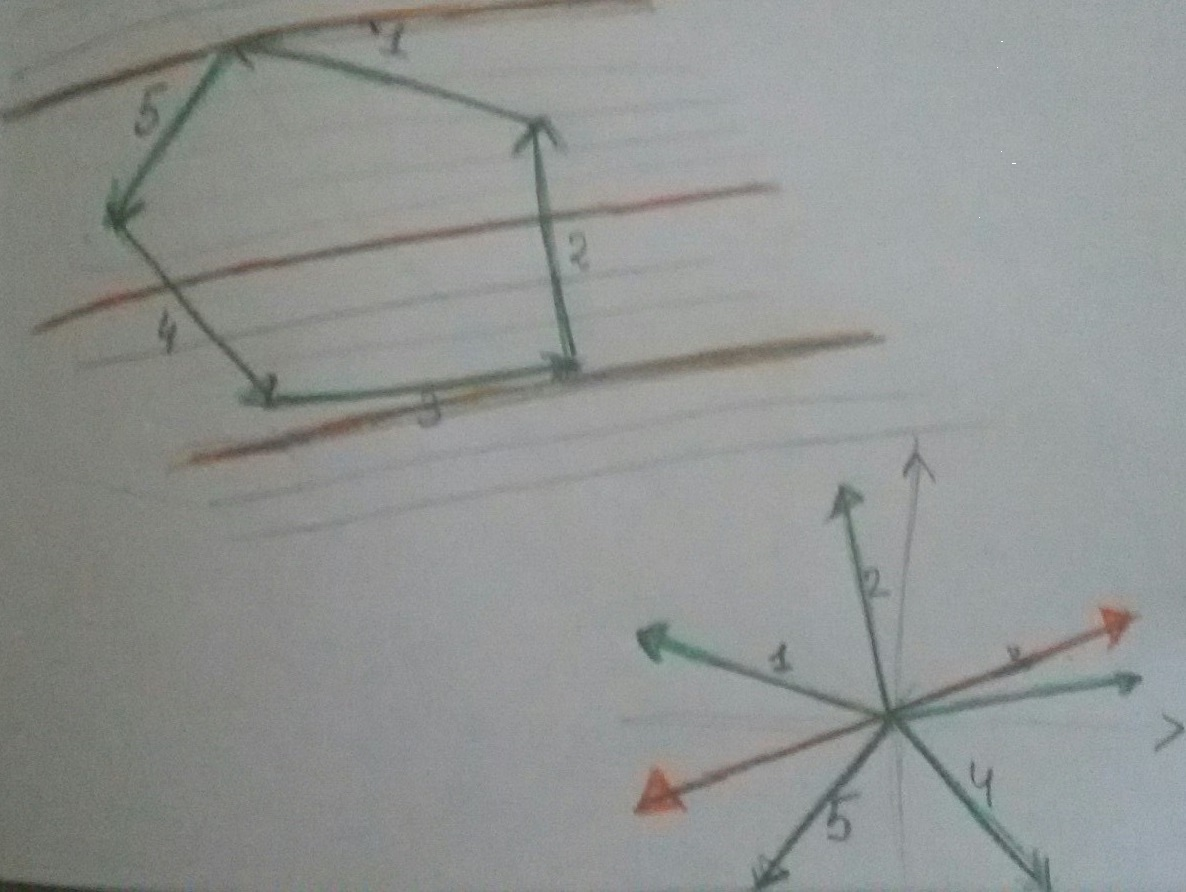
\includegraphics[width=2in, keepaspectratio]{im01.jpg} 
\end{center}

Можно, понятно как, за линию.

Теперь рассмотрим кучу параллельных прямых данной прямой. Какие-то прямые пересекаются, какие-то нет.
Если мы найдем параллельные касательные к многоугольнику, тогда
Нужно проверить, что прямая лежит между касательными.

Так как многоугольник выпуклый, то вектора, задающие стороны, из точки, будут идти покругу.

Как найти касательную?

Рассмотрим напровляющие вектора сторон и перенесем их в начало координат. 
Посмотрим на направляющий вектор прямой. Он находится между первым и пятым вектором и касательная находится между первой и пятой стороной.

Теперь, просто так по векторному углу сортировать нельзя, поскольку вектора есть как и с верхней стороны, так и с нижней. 

Нужно отдельно смотреть, вектора из одной полуплоскости или из разных.

Дальше, загоняем все в массив и делаем lower\_bound.

Что бы найти непосредственно точки пересечения с многоуголником, нужно сделать бинпоиск по границе с помощью орентированного расстояния.

\section{Существуют ли пересекающиеся отрезки} 

Идем сканлайном, порядок  непересекающихся отрезков не меняется. При появление нового отрезка, понятно в какое место его вставить. 

Теперь давай-те подумаем, где у нас могут появиться кандидаты на пересечение. Логично, что при добавление нового
отрезка нужно проверить, что он не пересечется с соседями. 

Не соседи могут пересечься только, если между ними никого нет. Точнее пересекаться могут, но не сейчас. 

То есть, при удаление отрезка нужно проверить, что новые соседи не пересекаются. 

События сканлайна
\begin{enumerate}
\item открылся отрезок
\item закрылся отрезок
\end{enumerate}
Сортируем события по x, если x одинаковый, то сначала отрезки будут открываться.

У нас будет \cpp"set<segment>"

В этом сете нужно с помощью lower\_bound найти соседние отрезки, проверяем и добавляем в нужное место.

Каждый раз проверяем максимум две пары.

При удаление, проверяем соседей и удаляем 

Компоратор в set

\begin{cppcode}

class cmp{ 
    bool operator() (segmetn s1, segment s2) {
        ...
    }
};

set <segment, cmp>
\end{cppcode}

Работает за $O(n \log n)$

Что делать с вертикальными прямыми? Сделаем вертикальную почти вертикальной, отклоним на эпсилон. То есть у прямой будет x и y.
